\documentclass[12pt,letterpaper]{article}
\usepackage[utf8]{inputenc}
\usepackage{amsmath}
\usepackage{amsfonts}
\usepackage{amssymb}
\usepackage{amsthm}
\usepackage{graphicx}
\usepackage[left=2cm,right=2cm,top=2cm,bottom=2cm]{geometry}
\author{Kris Garrett}
\title{Sweeps using Linear DG on Tetrahedra}
\begin{document}
\maketitle

Want to solve
\begin{equation}
\Omega \cdot \nabla_x f + \sigma_t f = Q
\end{equation}
via linear DG on tetrahedra.
Each DG basis is linear on a given cell $C$ and $0$ outside cell $C$.
There are four basis elements in a given cell $C$ which will be denoted $b_0, b_1, b_2, b_3$.
The interpolatory basis defined by $b_i(x_j) = \delta_{ij}$ where $x_j$ are the four vertices of the tetrahedron $C$ will be used.
Some preliminary facts will be needed.


\paragraph{Fact 1}
On a triangle $T$, the integral of a linear function $\ell$ which evaluates to 1 at one vertex and 0 at the other two vertices has integral
\begin{equation}
\int_T \ell dx = \frac{1}{3} A
\end{equation}
where $A$ is the area of the triangle.
\begin{proof}
Orient the triangle so that the vertex with evaluation $1$ is at $(0,0)$ and the opposite edge is parallel to the x-axis.
Below is a picture of such an orientation.
\begin{center}
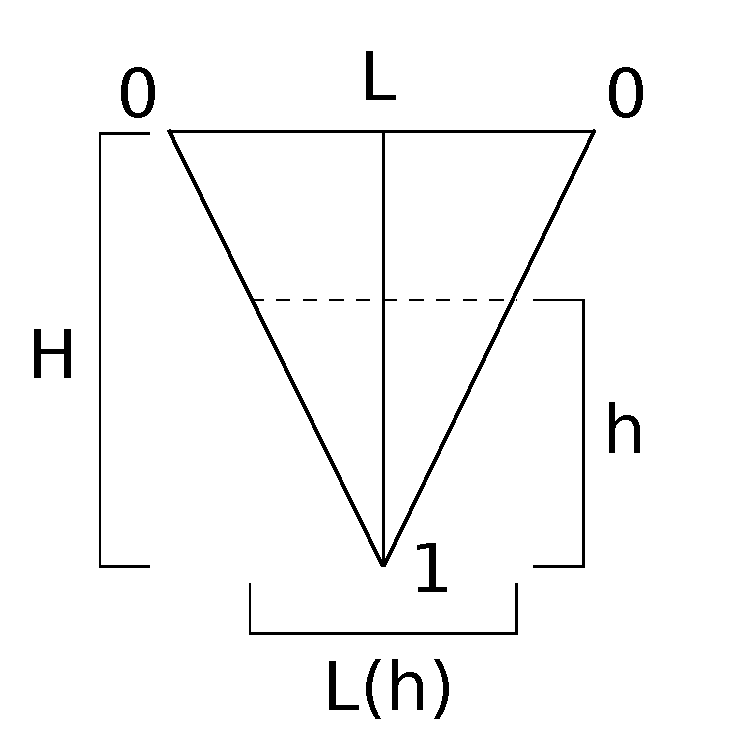
\includegraphics[scale=0.4]{triangle1.pdf}
\end{center}
Then, since $\ell$ is constant over $L(h)$ for any $h$
\begin{equation}
\int_T \ell \, dx = \int_0^H \int_{L(h)} \ell \, dL \, dh = \int_0^H \ell(0,h) L(h) \, dh
\end{equation}
with $\ell(0,h) = 1 - \frac{h}{H}$ and $L(h) = L \frac{h}{H}$.
Evaluating the integral leads to
\begin{align*}
\int_T \ell \, dx &= \int_0^H \ell(0,h) L(h) \, dh \\
&= \int_0^H \left(1 - \frac{h}{H} \right) L \frac{h}{H} \, dh \\
&= L H \int_0^1 (1 - u) u \, du \\
&= L H \left( \frac{1}{2} - \frac{1}{3} \right) = \frac{1}{6} L H = \frac{1}{3} A.
\end{align*}
\end{proof}


\paragraph{Fact 2}
On a triangle $T$, the integral of $\ell_i \ell_j$ where $\ell_k$ is a linear function which evaluates to 1 at vertex $k$ and 0 at the other two vertices has integral
\begin{equation}
\int_T \ell_i \ell_j dx = \begin{cases}
\frac{1}{12} A, \qquad &\textrm{if } i \neq j \\
\frac{1}{6} A, \qquad &\textrm{if } i = j. \\
\end{cases}
\end{equation}
\begin{proof}
Suppose $i = j$.
Then the proof is similar to the one in Fact 1, but $\ell(0,h)$ is replaced with its square
\begin{align*}
\int_T \ell_i^2 \, dx &= \int_0^H \ell(0,h)^2 L(h) \, dh \\
&= \int_0^H \left(1 - \frac{h}{H} \right)^2 L \frac{h}{H} \, dh \\
&= L H \int_0^1 (1 - u)^2 u \, du \\
&= L H \left( \frac{1}{2} - \frac{2}{3} + \frac{1}{4} \right) = \frac{1}{12} L H = \frac{1}{6} A.
\end{align*}

Now suppose $i \neq j$.
Use the same idea for the proof as in Fact 1 with $\ell_i$ evaluating to 1 at the bottom vertex.
This means $\ell_j$ evaluates to 1 at one of the top vertices.
The integral is given by
\begin{equation}
\int_T \ell_i \ell_j \, dx 
= \int_0^H \int_{L(h)} \ell_i \ell_j \, dL \, dh 
= \int_0^H \ell_i(0,h) \int_{L(h)} \ell_j \, dL \, dh
\end{equation}
since $\ell_i$ is constant on $L(h)$.
On $L(h)$, $\ell_j$ evaluates to zero at one end and $\frac{h}{H}$ at the other end.
This makes the integral
\begin{equation}
\int_{L(h)} \ell_j \, dL = \frac{1}{2} \frac{h}{H} L(h) = \frac{L}{2} \left( \frac{h}{H} \right)^2.
\end{equation}
Therefore
\begin{align}
\int_T \ell_i \ell_j \, dx 
&= \int_0^H \ell_i(0,h) \frac{L}{2} \left( \frac{h}{H} \right)^2 \, dh \\
&= \int_0^H \left(1 - \frac{h}{H} \right) \frac{L}{2} \left( \frac{h}{H} \right)^2 \, dh \\
&= \frac{1}{2} LH \int_0^1 \left(1 - u \right) u^2 \, du \\
&= \frac{1}{2} LH \left( \frac{1}{3} - \frac{1}{4} \right) = \frac{1}{12} A.
\end{align}
\end{proof}


\paragraph{Fact 3}
On a tetrahedron cell $C$, the integral of a linear function $\ell$ which evaluates to 1 at one vertex and 0 at the other three vertices has integral
\begin{equation}
\int_T \ell dx = \frac{1}{4} V
\end{equation}
where $V$ is the volume of $C$.
\begin{proof}
Orient the cell so that the vertex with evaluation $1$ is at the origin and the opposite face is parallel and above the x,y-axes.
Below is a picture of such an orientation.
\begin{center}
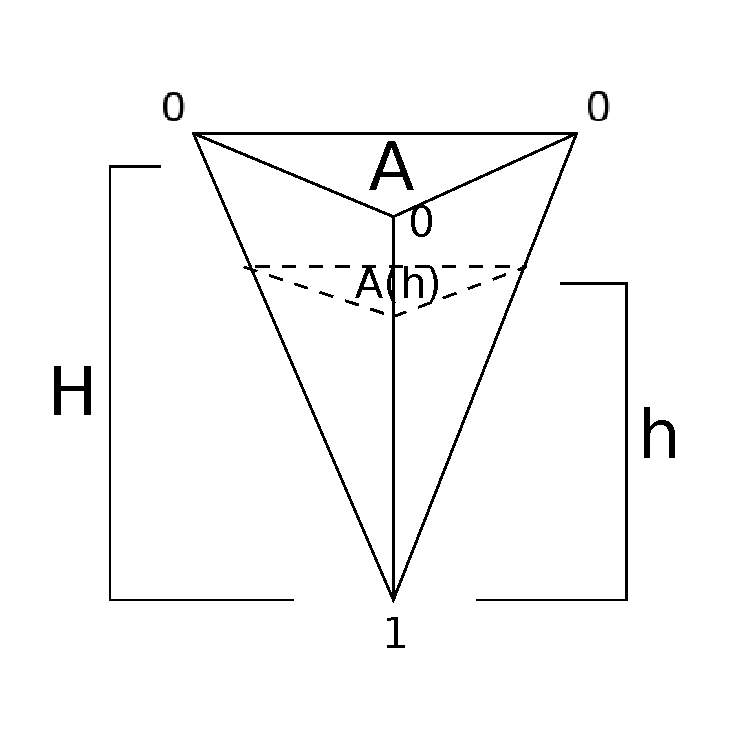
\includegraphics[scale=0.6]{tet1.pdf}
\end{center}
Then using similar logic as before
\begin{equation}
\int_C \ell \, dx = \int_0^H \int_{A(h)} \ell \, dA \, dh = \int_0^H \ell(0,0,h) A(h) \, dh
\end{equation}
with $\ell(0,0,h) = 1 - \frac{h}{H}$ and $A(h) = A \frac{h^2}{H^2}$.
Evaluating the integral leads to
\begin{align*}
\int_C \ell \, dx &= \int_0^H \ell(0,0,h) A(h) \, dh \\
&= \int_0^H \left( 1 - \frac{h}{H} \right) A \frac{h^2}{H^2} \, dh \\
&= A H \int_0^1 (1 - u) u^2 \, du \\
&= A H \left( \frac{1}{3} - \frac{1}{4} \right) = \frac{1}{12} A H = \frac{1}{4} V.
\end{align*}
\end{proof}


\paragraph{Fact 4}
On a tetrahedron cell $C$, the integral of the multiplication of two linear functions $\ell_i$, $\ell_j$ which evaluate to 1 at one vertex and 0 at the other three vertices has integral
\begin{equation}
\int_C \ell_i \ell_j dx = \begin{cases}
\frac{1}{20} V, \qquad \textrm{if } i \neq j \\
\frac{1}{10} V, \qquad \textrm{if } i = j \\
\end{cases}
\end{equation}
where $V$ is the volume of $C$.
\begin{proof}
Suppose $i = j$.
Then the integral is calculated as in Fact 3
\begin{align*}
\int_C \ell_i^2 dx &= \int_0^H \ell_i(0,0,h)^2 A(h) \, dh \\
&= \int_0^H \left(1 - \frac{h}{H} \right)^2 A \frac{h^2}{H^2} \, dh \\
&= A H \int_0^1 (1 - u)^2 u^2 \, du \\
&= A H \left(\frac{1}{3} - \frac{1}{2} + \frac{1}{5}\right) = \frac{1}{30} A H = \frac{1}{10} V.
\end{align*}

Suppose $i \neq j$.
Orient the cell so that $\ell_i$ evaluate to $1$ at $(0,0,0)$ and the opposite face is parallel to the x,y-axes.
Then $\ell_j$ will evaluate to 1 at one of the top vertices.
This leads to
\begin{align*}
\int_C \ell_1 \ell_2 \, dx &= \int_0^H \ell_1(0,0,h) \int_{T(h)} \ell_2 \, dA \, dh \\
&= \int_0^H \left(1 - \frac{h}{H}\right) \frac{1}{3} \frac{h}{H} A(h) \, dh \\
&= \int_0^H \left(1 - \frac{h}{H}\right) \frac{1}{3} \frac{h}{H} A \frac{h^2}{H^2} \, dh \\
&= \frac{1}{3} A H \int_0^1 (1 - u) u^3 \, du \\
&= \frac{1}{3} A H \left(\frac{1}{4} - \frac{1}{5}\right) = \frac{1}{20} V.
\end{align*}
Line 1 to 2 above follows from Fact 1 and the fact that $\ell_j$ at height $h$ has vertices evaluate to $0$, $0$ and $\frac{h}{H}$.
\end{proof}


\section*{DG Equations}
Now to solve the sweep equations with linear DG.
The governing equation is
\begin{equation}
\Omega \cdot \nabla_x f + \sigma_t f = Q.
\end{equation}
Apply test function $b_j$ with $j = 0,1,2,3$ on C
\begin{equation}
\int_C \Omega \cdot \nabla_x f b_j dx + \int_C \sigma_t f b_j dx = \int_C Q b_j dx.
\end{equation}
Integrate by parts
\begin{equation}
-\int_C \Omega \cdot \nabla_x b_j f dx + \sum_k \int_{F_k} (\Omega \cdot \nu_k) b_j \hat{f} dA + \int_C \sigma_t f b_j dx = \int_C Q b_j dx
\end{equation}
where $F_k$ for $k = 0,1,2,3$ is the faces of cell $C$ and $\nu_k$ is the outward normal to $F_k$.
The hat on the $f$ represents the fact that $f$ on the boundary is not well-defined (since $f$ can be discontinuous at the boundary) so the approximation scheme must define it.
This paper will assume upwind fluxes defined as
\begin{equation}
\hat{f} = \begin{cases}
\textrm{f from C}, \qquad &\textrm{if } \Omega \cdot \nu_k > 0 \\
\textrm{f from cell adjacent to C}, \qquad &\textrm{if } \Omega \cdot \nu_k < 0. \\
\end{cases}
\end{equation}
Write $$f = f_0 b_0 + f_1 b_1 + f_2 b_2 + f_3 b_3 \qquad \textrm{and} \qquad Q = Q_0 b_0 + Q_1 b_1 + Q_2 b_2 + Q_3 b_3.$$
Then write the flux $$\hat{f}|_{F_k} = \hat{f}^{(k)}_0 b_0 + \hat{f}^{(k)}_1 b_1 + \hat{f}^{(k)}_2 b_2 + \hat{f}^{(k)}_3 b_3.$$
Denote $A_j$ the area of face $j$, $V$ the volume of cell $C$, and $\bar{A}_j = (\Omega \cdot \nu_j) A_j$.

\paragraph{Equation}
\begin{equation}
\int_C f b_j dx = \sum_i \int_C f_i b_i b_j dx
= \frac{1}{20} V (f_0 + f_1 + f_2 + f_3 + f_j)
\end{equation}

\paragraph{Equation} Similarly
\begin{equation}
\int_C Q b_j dx = \frac{1}{20} V (Q_0 + Q_1 + Q_2 + Q_3 + Q_j)
\end{equation}

\paragraph{Equation}
Note that $\Omega \cdot \nabla_x$ is a directional derivative in direction $\Omega$.
Split the directional derivative in two with one direction parallel to $\nu_j$ and the other perpendicular to $\nu_j$
\begin{equation}
\Omega \cdot \nabla_x = (\Omega \cdot \nu_j) \nu_j \cdot \nabla_x + \Omega^\perp \cdot \nabla_x.
\end{equation}
The point of this is $\Omega^\perp \cdot \nabla_x b_j = 0$ and $\nu_j \cdot \nabla_x b_j = \frac{1}{L_j}$ where $L_j$ is the height of the tetrahedron perpendicular to face $j$.
Then using $\frac{1}{3} L_j A_j = V$
\begin{align}
\int_C \Omega \cdot \nabla_x b_j f dx &= \sum_i \int_C (\Omega \cdot \nu_j) \frac{1}{L_j} f_i b_i dx \\
&= \sum_i \frac{1}{4} V f_i (\Omega \cdot \nu_j) \frac{1}{L_j} \\
&= \sum_i \frac{1}{12} f_i (\Omega \cdot \nu_j) A_j = \frac{1}{12} \bar{A}_j (f_0 + f_1 + f_2 + f_3).
\end{align}

\paragraph{Equation}
\begin{equation}
\sum_k \int_{F_k} (\Omega \cdot \nu_k) b_j \hat{f} dA = \sum_{i,k} \hat{f}^{(k)}_i (\Omega \cdot \nu_k) \int_{\partial F_k} b_j b_i dA
\end{equation}
If $j = k$ or $i = k$ then the integral is zero since either $b_i$ or $b_j$ is zero on the triangle.
In the case $j \neq k$ and $i \neq k$, one can use Fact 2.
This yields
\begin{equation}
\sum_k \int_{F_k} (\Omega \cdot \nu_k) b_j \hat{f} dA = \sum_{i \neq k, j \neq k} \begin{cases}
\frac{1}{12} \hat{f}^{(k)}_i \bar{A}_k, \qquad &\textrm{if } i \neq j \\
\frac{1}{6} \hat{f}^{(k)}_i \bar{A}_k, \qquad &\textrm{if } i = j \\
\end{cases}
\end{equation}


\paragraph{Putting it all together}
Putting all the equations together leads to a system of 4 equations, one per test function $b_j$.
The equations are:
\begin{align*}
\frac{1}{12} \bar{A}_1 \left( 2\hat{f}^{(1)}_0 + \hat{f}^{(1)}_2 + \hat{f}^{(1)}_3 \right)
+ \frac{1}{12} \bar{A}_2 \left( 2\hat{f}^{(2)}_0 + \hat{f}^{(2)}_1 + \hat{f}^{(2)}_3 \right)
+ \frac{1}{12} \bar{A}_3 \left( 2\hat{f}^{(3)}_0 + \hat{f}^{(3)}_1 + \hat{f}^{(3)}_2 \right) \\
+ \frac{1}{12} \bar{A}_0 \left( f_0 + f_1 + f_2 + f_3 \right)
+ \frac{\sigma_t V}{20} \left( 2f_0 + f_1 + f_2 + f_3 \right)
+ \frac{V}{20} \left( 2Q_0 + Q_1 + Q_2 + Q_3 \right)
\end{align*}
\begin{align*}
\frac{1}{12} \bar{A}_0 \left( 2\hat{f}^{(1)}_1 + \hat{f}^{(1)}_2 + \hat{f}^{(1)}_3 \right)
+ \frac{1}{12} \bar{A}_2 \left( \hat{f}^{(2)}_0 + 2\hat{f}^{(2)}_1 + \hat{f}^{(2)}_3 \right)
+ \frac{1}{12} \bar{A}_3 \left( \hat{f}^{(3)}_0 + 2\hat{f}^{(3)}_1 + \hat{f}^{(3)}_2 \right) \\
+ \frac{1}{12} \bar{A}_1 \left( f_0 + f_1 + f_2 + f_3 \right)
+ \frac{\sigma_t V}{20} \left( f_0 + 2f_1 + f_2 + f_3 \right)
+ \frac{V}{20} \left( Q_0 + 2Q_1 + Q_2 + Q_3 \right)
\end{align*}
\begin{align*}
\frac{1}{12} \bar{A}_0 \left( \hat{f}^{(1)}_1 + 2\hat{f}^{(1)}_2 + \hat{f}^{(1)}_3 \right)
+ \frac{1}{12} \bar{A}_1 \left( \hat{f}^{(2)}_0 + 2\hat{f}^{(2)}_2 + \hat{f}^{(2)}_3 \right)
+ \frac{1}{12} \bar{A}_3 \left( \hat{f}^{(3)}_0 + \hat{f}^{(3)}_1 + 2\hat{f}^{(3)}_2 \right) \\
+ \frac{1}{12} \bar{A}_2 \left( f_0 + f_1 + f_2 + f_3 \right)
+ \frac{\sigma_t V}{20} \left( f_0 + f_1 + 2f_2 + f_3 \right)
+ \frac{V}{20} \left( Q_0 + Q_1 + 2Q_2 + Q_3 \right)
\end{align*}
\begin{align*}
\frac{1}{12} \bar{A}_0 \left( \hat{f}^{(1)}_1 + \hat{f}^{(1)}_2 + 2\hat{f}^{(1)}_3 \right)
+ \frac{1}{12} \bar{A}_1 \left( \hat{f}^{(2)}_0 + \hat{f}^{(2)}_2 + 2\hat{f}^{(2)}_3 \right)
+ \frac{1}{12} \bar{A}_2 \left( \hat{f}^{(3)}_0 + \hat{f}^{(3)}_1 + 2\hat{f}^{(3)}_3 \right) \\
+ \frac{1}{12} \bar{A}_3 \left( f_0 + f_1 + f_2 + f_3 \right)
+ \frac{\sigma_t V}{20} \left( f_0 + f_1 + f_2 + 2f_3 \right)
+ \frac{V}{20} \left( Q_0 + Q_1 + Q_2 + 2Q_3 \right)
\end{align*}


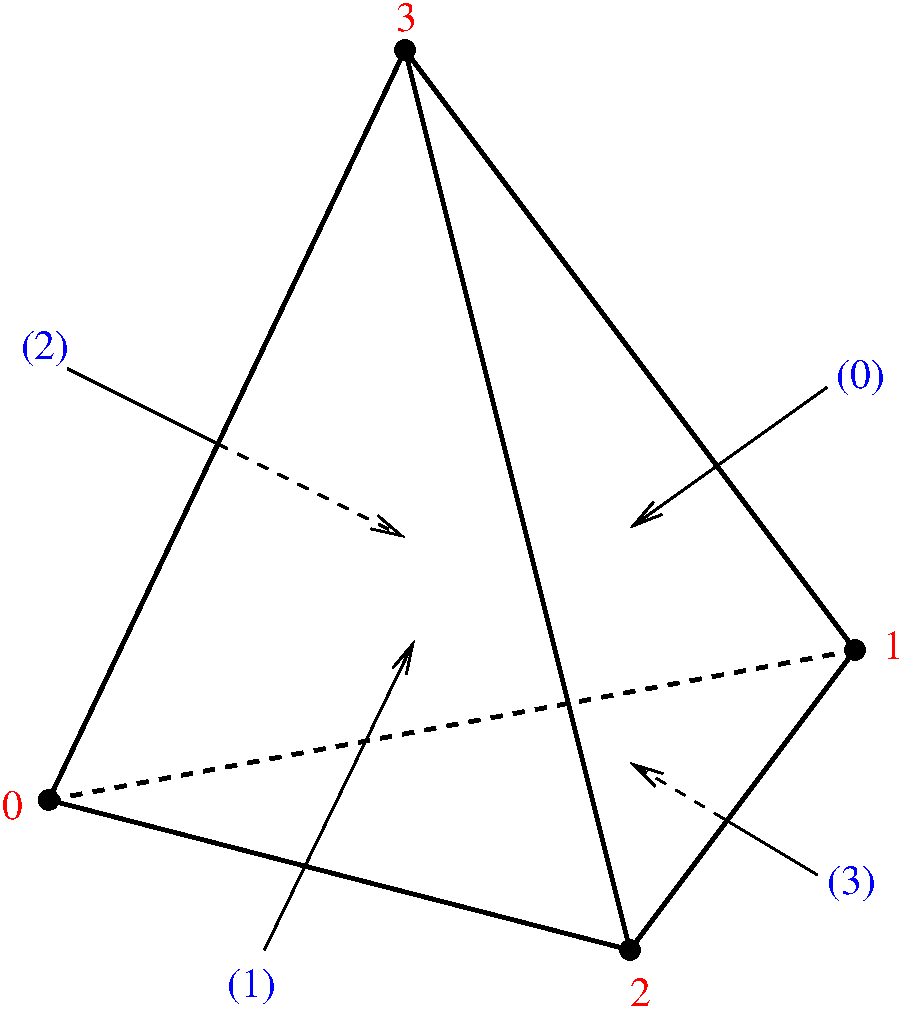
\includegraphics[scale=0.5]{tet-eps-converted-to.pdf}



\end{document}